\renewcommand{\theequation}{\theenumi}
\begin{enumerate}[label=\arabic*.,ref=\thesubsection.\theenumi]
\numberwithin{equation}{enumi}

\item Let 
\begin{align}
\vec{x} = \myvec{a\\0}
\end{align}
%
Substituting in \eqref{eq:p1}, 
%
\begin{align}
\myvec{1 & -1} \myvec{a\\0}&= -1
\\
\implies a &=-1
\end{align}
%
Simiarly, substituting 
%
\begin{align}
\vec{x} &= \myvec{0\\b},
\end{align}
%
in \eqref{eq:p1}, 
%
%
\begin{align}
b =1
\end{align}
%
The intercepts on the x and y-axis from above are 
\begin{align}
\vec{A} = \myvec{-1\\0}
\vec{B} = \myvec{0\\1}
\end{align}
The python code for the Problem \eqref{eq:p1}
%
can be used to plot Fig. \ref{fig:intercept1}.
%
\begin{figure}[!ht]
\includegraphics[width=\columnwidth]{./figs/triangle/icept1.eps}
\caption{Intercept 1}
\label{fig:intercept1}
\end{figure}

\label{eq:p1xaxis}
$\vec{A}$ is the x-intercept of the line and is the point where it meets x-axis.
\\
Using the above method, the intercepts on x and y-axis for the equation .\eqref{eq:p2} are
\begin{align}
\vec{C} = \myvec{4\\0}
\vec{D} = \myvec{0\\6}
\end{align}

\label{eq:p2xaxis}
$\vec{C}$ is the x-intercept of the line and is the point where it meets x-axis.
The python code for the Problem \eqref{eq:p2}
%
can be used to plot Fig. \ref{fig:intercept2}.
%
\begin{figure}[!ht]
\includegraphics[width=\columnwidth]{./figs/triangle/icept2.eps}
\caption{Intercept 2}
\label{fig:intercept2}
\end{figure}

The above equations can be expressed as the matrix equation
\begin{align}
\myvec{1 & -1\\3 & 2} \vec{x} = \myvec{-1\\12}
\end{align}
%
The augmented matrix for the above equation is row reduced as follows
\begin{align}
\myvec{1 & -1 & -1\\3 & 2 & 12} 
\xleftrightarrow {R_2\leftarrow \frac{R_2-3R_1}{5}}\myvec{1 & -1 & -1\\0 & 1 & 3} 
\\
%\myvec{1 & -1 & -1\\0 & 1 & 3} 
\xleftrightarrow {R_1\leftarrow R_1 + R_2}\myvec{1 & 0 & 2\\0 & 1 & 3} 
\label{eq:line_aug}
\end{align}
%
$\implies \vec{x}=\myvec{2\\3}$
The equivalent python code is
%
\begin{lstlisting}
codes/triangle/line_intersect.py
\end{lstlisting}
%
which plots Fig. \ref{fig:line_intercept}, intersect at $\myvec{2\\3}$
%
\begin{figure}[!ht]
\includegraphics[width=\columnwidth]{./figs/triangle/line_intercept.eps}
\caption{Line intercept}
\label{fig:line_intercept}
\end{figure}

\item And the vertices of triangle \eqref{fig:Shaded} formed due to the intersection of lines and x-axis are:
\begin{align}
\vec{A}=\myvec{2\\3}
\\
\vec{B}=\myvec{-1\\0}
\\
\vec{C}=\myvec{4\\0}
\end{align}
Where $\vec{B}$ and $\vec{C}$ are X-intercepts of line \eqref{eq:p1} and \eqref{eq:p2} respectively (from \eqref{eq:p1xaxis} and \eqref{eq:p2xaxis}).
\begin{figure}[!ht]
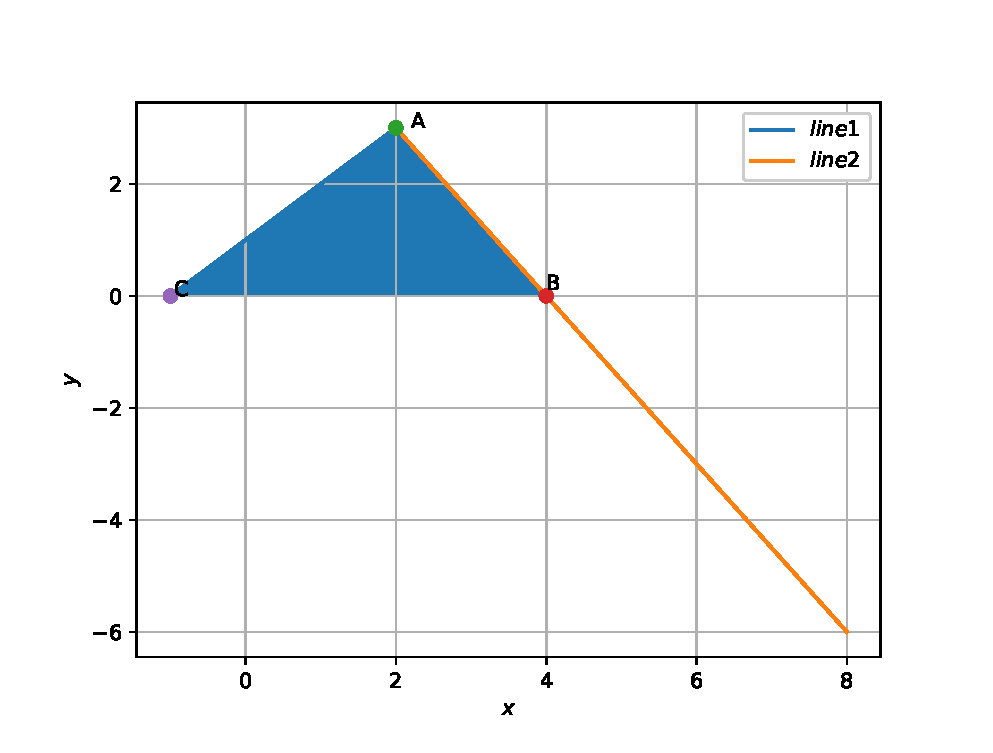
\includegraphics[width=\columnwidth]{./figs/triangle/shaded.eps}
\caption{Shaded Triangle}
\label{fig:Shaded}
\end{figure}
The equivalent python code for figure \eqref{fig:Shaded} is
%
\begin{lstlisting}
codes/triangle/shaded.py
\end{lstlisting}

\end{enumerate}